% Preamble: \usepackage{graphicx,array}
\setlength{\tabcolsep}{0.5pt}
\renewcommand{\arraystretch}{1.0}

\begin{figure}[t]
\centering
\newcommand{\imgw}{0.24\linewidth} % 4 images × 0.24 = 0.96 (safe)
\begin{tabular}{@{}cccc@{}}
  % Header
  % \multicolumn{4}{@{}l@{}}{{\scriptsize\textbf{Structured edits (disentanglement)}}} \\[-1pt]

  % Images (row)
  % \multicolumn{4}{c}{\textit{``A mother duck guards three rubber duckies.''}} \\
  % \multicolumn{4}{c}{\textit{``A bouquet of  flowers is upside down in a vase.''}} \\
  % \includegraphics[width=\imgw]{Figures/contextual_contradictions/images/vase/flux.png} &
  % \includegraphics[width=\imgw]{Figures/contextual_contradictions/images/vase/hidream.jpg} &
  % \includegraphics[width=\imgw]{Figures/contextual_contradictions/images/vase/qwen.jpg} &
  % 
\includegraphics[width=\imgw]{Figures/contextual_contradictions/images/vase/bria_new.jpg}
  % \\[-2pt]

    % Images (row)
      \multicolumn{4}{c}{\textit{``A bear is performing a
handstand in the park.''}} \\
  \includegraphics[width=\imgw]{Figures/contextual_contradictions/images/bear/flux.png} &
  \includegraphics[width=\imgw]{Figures/contextual_contradictions/images/bear/hidream.jpg} &
  \includegraphics[width=\imgw]{Figures/contextual_contradictions/images/bear/qwen.jpg} &
  \includegraphics[width=\imgw]{Figures/contextual_contradictions/images/bear/bria_new_new.jpg}
  \\%[-2pt]

    % Images (row)

    \multicolumn{4}{c}{\textit{``A woman writing with a dart.''}} \\
  \includegraphics[width=\imgw]{Figures/contextual_contradictions/images/woman_dart/flux.png} &
  \includegraphics[width=\imgw]{Figures/contextual_contradictions/images/woman_dart/hidream.jpg} &
  \includegraphics[width=\imgw]{Figures/contextual_contradictions/images/woman_dart/qwen.jpg} &
  \includegraphics[width=\imgw]{Figures/contextual_contradictions/images/woman_dart/bria_new_new.jpg}
  \\%[-2pt]
  
  %  \multicolumn{4}{c}{\textit{``A balloon is lifting up a package.''}} \\
  % \includegraphics[width=\imgw]{Figures/contextual_contradictions/images/ballon/flux.jpg} &
  % \includegraphics[width=\imgw]{Figures/contextual_contradictions/images/ballon/hidream.jpg} &
  % \includegraphics[width=\imgw]{Figures/contextual_contradictions/images/ballon/qwen.jpg} &
  % 
\includegraphics[width=\imgw]{Figures/contextual_contradictions/images/ballon/bria_new.jpeg}

  % \\%[-2pt]

% \multicolumn{4}{c}{\textit{``A butterfly is in a bee’s hive.''}} \\
%   \includegraphics[width=\imgw]{Figures/contextual_contradictions/images/butterfly_hive/flux.jpg} &
%   \includegraphics[width=\imgw]{Figures/contextual_contradictions/images/butterfly_hive/hidream.jpg} &
%   \includegraphics[width=\imgw]{Figures/contextual_contradictions/images/butterfly_hive/qwen.jpg} &
%   \includegraphics[width=\imgw]{Figures/contextual_contradictions/images/butterfly_hive/bria_new_3.jpg}

%   \\%[-2pt]

\multicolumn{4}{c}{\textit{``A professional boxer does a split.''}} \\
  \includegraphics[width=\imgw]{Figures/contextual_contradictions/images/boxer/flux.jpg} &
  \includegraphics[width=\imgw]{Figures/contextual_contradictions/images/boxer/hidream.jpg} &
  \includegraphics[width=\imgw]{Figures/contextual_contradictions/images/boxer/qwen.jpg} &
  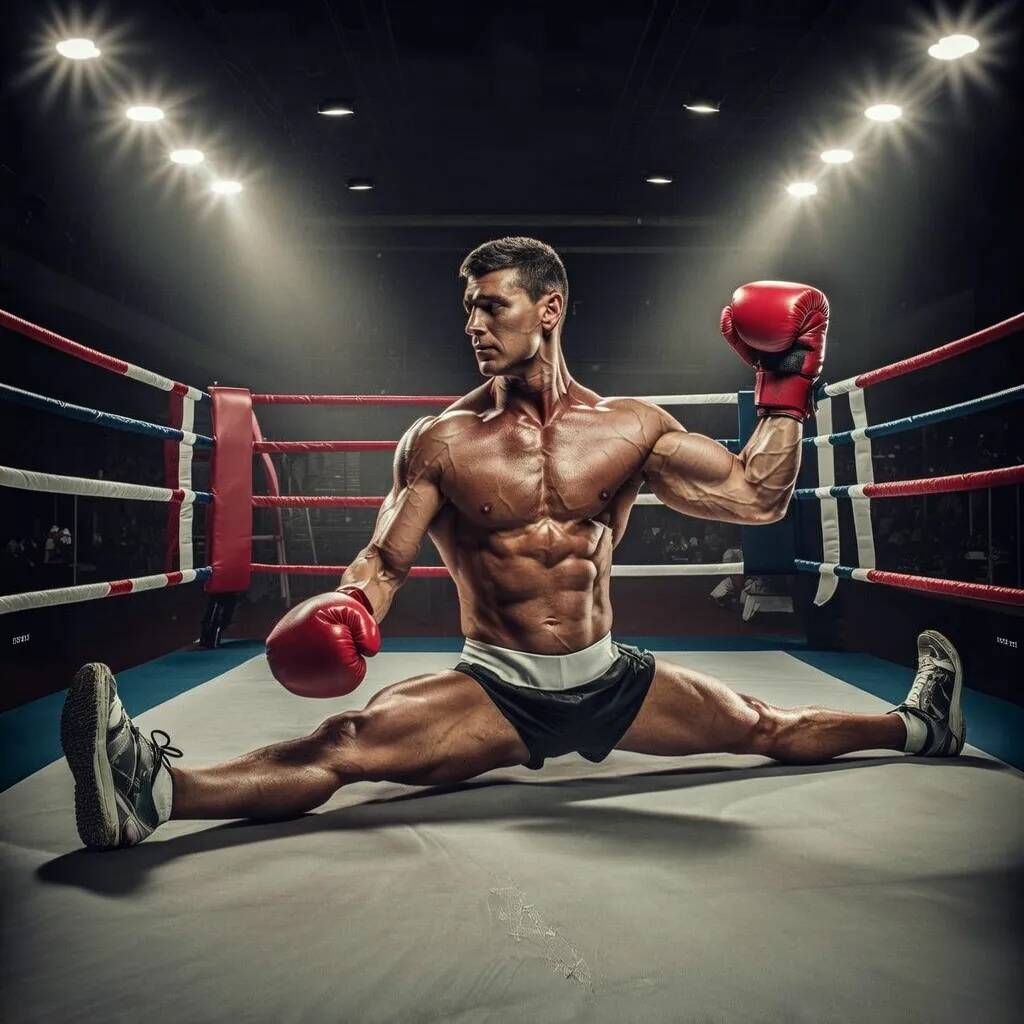
\includegraphics[width=\imgw]{Figures/contextual_contradictions/images/boxer/bria_new.jpeg}

  \\%[-2pt]


  % Wrapped labels under each image (row)
  \parbox{\imgw}{\scriptsize\centering \textbf{FLUX}} &
  \parbox{\imgw}{\scriptsize\centering \textbf{HiDream}} &
  \parbox{\imgw}{\scriptsize\centering \textbf{Qwen-Image}} &
  \parbox{\imgw}{\scriptsize\centering \textbf{Fibo (Ours)}}
  \\
\end{tabular}

\vspace{-3pt}
\caption{\textbf{Contextual contradiction.} We use prompts from ContraBench~\cite{huberman2025image} and Whoops~\cite{Bitton_Guetta_2023}. \modelname{} generates semantically consistent images that faithfully represent the correct relations, unlike other models that often default to typical co-occurrences. }
\label{fig:contextual}
\end{figure}